\documentclass[11pt]{article}
\usepackage[margin=0.8in]{geometry}
\usepackage{amsmath,amssymb,booktabs,array,longtable}
\usepackage{hyperref}
\usepackage{enumitem}
\usepackage{graphicx}
\usepackage{float}
\usepackage{caption}
\usepackage{tikz}
\usetikzlibrary{positioning,arrows.meta}
\setlist{nosep}

\begin{document}

\begin{center}
{\Large\textbf{Shiv Nadar University Chennai}}\\
\textbf{CS3807 -- Deep Learning Laboratory}\\
\textbf{Experiment 3}\\
{\large\textbf{Implementation of Convolutional Neural Networks (CNNs) for Image Classification}}
\end{center}

\renewcommand{\arraystretch}{1.25}

\begin{tabular}{|p{3.8cm}|p{8cm}|p{2cm}|}
\hline
Degree \& Branch & B.Tech Artificial Intelligence \& Data Science & Semester V\\ \hline
Subject Code \& Name & CS3807 -- Deep Learning Laboratory & AY: 2026--27\\ \hline
\end{tabular}

\section*{1. Objective}

To understand the working principle of Convolutional Neural Networks by implementing convolution, pooling, feature map visualization, and image classification using TensorFlow/Keras.

\section*{2. Learning Outcomes}

Students will be able to

\begin{enumerate}
\item Explain the convolution operation.
\item Compute output dimensions using stride and padding.
\item Visualize feature maps.
\item Implement max pooling and average pooling.
\item Calculate CNN parameters.
\item Build a CNN for image classification.
\item Evaluate CNN performance.
\end{enumerate}

\section*{3. Background Theory}

A Convolutional Neural Network consists of

\begin{itemize}
\item Convolution Layer
\item Activation Layer
\item Pooling Layer
\item Fully Connected Layer
\end{itemize}

The convolution operation is

\[
Y(i,j)=\sum_m\sum_n X(i+m,j+n)K(m,n)
\]

where

\begin{itemize}
\item $X$ : Input Image
\item $K$ : Kernel (Filter)
\item $Y$ : Feature Map
\end{itemize}

The output feature map size is

\[
\frac{N-F+2P}{S}+1
\]

where

\begin{tabular}{ll}
$N$ & Input Size\\
$F$ & Filter Size\\
$P$ & Padding\\
$S$ & Stride
\end{tabular}

\subsection*{3.1 Common Convolution Kernels}

A \textbf{kernel} (or \textbf{filter}) is a small matrix that slides over an input image to extract important visual features such as edges, textures, corners, and smooth regions. During convolution, the kernel is multiplied element-wise with the corresponding image pixels, and the results are summed to produce a single value in the output feature map. Different kernels highlight different image characteristics.

\subsubsection*{1. Identity Kernel}

The identity kernel preserves the original image without modifying its pixel values.

\[
\begin{bmatrix}
0 & 0 & 0\\
0 & 1 & 0\\
0 & 0 & 0
\end{bmatrix}
\]

\textbf{Purpose:}
\begin{itemize}
\item Preserves the original image.
\item Used for understanding the convolution operation.
\end{itemize}

\subsubsection*{2. Sobel-X Kernel (Vertical Edge Detection)}

The Sobel-X kernel detects \textbf{vertical edges} by measuring intensity changes along the horizontal direction.

\[
\begin{bmatrix}
-1 & 0 & 1\\
-2 & 0 & 2\\
-1 & 0 & 1
\end{bmatrix}
\]

\textbf{Applications:}
\begin{itemize}
\item Object detection
\item Lane detection
\item Face recognition
\end{itemize}

\subsubsection*{3. Sobel-Y Kernel (Horizontal Edge Detection)}

The Sobel-Y kernel detects \textbf{horizontal edges} by measuring intensity changes along the vertical direction.

\[
\begin{bmatrix}
-1 & -2 & -1\\
0 & 0 & 0\\
1 & 2 & 1
\end{bmatrix}
\]

\textbf{Applications:}
\begin{itemize}
\item Text detection
\item Boundary extraction
\item Medical image analysis
\end{itemize}

\subsubsection*{4. Laplacian Kernel}

The Laplacian kernel detects edges in all directions using the second-order derivative of image intensity.

\[
\begin{bmatrix}
0 & -1 & 0\\
-1 & 4 & -1\\
0 & -1 & 0
\end{bmatrix}
\]

\textbf{Applications:}
\begin{itemize}
\item Edge enhancement
\item Satellite image analysis
\item Medical imaging
\end{itemize}

\subsubsection*{5. Sharpening Kernel}

This kernel enhances fine details by emphasizing high-frequency components.

\[
\begin{bmatrix}
0 & -1 & 0\\
-1 & 5 & -1\\
0 & -1 & 0
\end{bmatrix}
\]

\textbf{Applications:}
\begin{itemize}
\item Image enhancement
\item Optical Character Recognition (OCR)
\item Face recognition
\end{itemize}

\subsubsection*{6. Box Blur Kernel}

The Box Blur kernel smooths an image by replacing each pixel with the average of its neighboring pixels.

\[
\frac{1}{9}
\begin{bmatrix}
1 & 1 & 1\\
1 & 1 & 1\\
1 & 1 & 1
\end{bmatrix}
\]

\textbf{Applications:}
\begin{itemize}
\item Noise removal
\item Image smoothing
\item Image preprocessing
\end{itemize}

\subsubsection*{7. Gaussian Blur Kernel}

Gaussian blur smooths the image while preserving the overall structure better than a simple average filter.

\[
\frac{1}{16}
\begin{bmatrix}
1 & 2 & 1\\
2 & 4 & 2\\
1 & 2 & 1
\end{bmatrix}
\]

\textbf{Applications:}
\begin{itemize}
\item Noise reduction
\item Computer vision preprocessing
\item Feature extraction
\end{itemize}

\subsubsection*{8. Emboss Kernel}

The Emboss kernel creates a three-dimensional appearance by emphasizing directional changes in intensity.

\[
\begin{bmatrix}
-2 & -1 & 0\\
-1 & 1 & 1\\
0 & 1 & 2
\end{bmatrix}
\]

\textbf{Applications:}
\begin{itemize}
\item Texture analysis
\item Artistic image effects
\end{itemize}

\subsubsection*{9. Outline Detection Kernel}

This kernel highlights object boundaries by emphasizing regions with rapid intensity changes.

\[
\begin{bmatrix}
-1 & -1 & -1\\
-1 & 8 & -1\\
-1 & -1 & -1
\end{bmatrix}
\]

\textbf{Applications:}
\begin{itemize}
\item Image segmentation
\item Boundary detection
\item Shape extraction
\end{itemize}

\subsubsection*{10. Motion Blur Kernel}

This kernel simulates motion blur along the diagonal direction.

\[
\frac{1}{5}
\begin{bmatrix}
1 & 0 & 0 & 0 & 0\\
0 & 1 & 0 & 0 & 0\\
0 & 0 & 1 & 0 & 0\\
0 & 0 & 0 & 1 & 0\\
0 & 0 & 0 & 0 & 1
\end{bmatrix}
\]

\textbf{Applications:}
\begin{itemize}
\item Motion simulation
\item Image restoration
\item Video processing
\end{itemize}

\subsubsection*{Summary of Common Kernels}

\begin{center}
\renewcommand{\arraystretch}{1.3}
\begin{tabular}{|p{3cm}|p{2cm}|p{4cm}|p{4cm}|}
\hline
\textbf{Kernel} & \textbf{Size} & \textbf{Purpose} & \textbf{Applications}\\
\hline
Identity & $3\times3$ & Preserve original image & Baseline comparison\\
\hline
Sobel-X & $3\times3$ & Detect vertical edges & Object detection\\
\hline
Sobel-Y & $3\times3$ & Detect horizontal edges & Boundary detection\\
\hline
Laplacian & $3\times3$ & Detect edges in all directions & Medical imaging\\
\hline
Sharpen & $3\times3$ & Enhance details & Image enhancement\\
\hline
Box Blur & $3\times3$ & Smooth image & Noise removal\\
\hline
Gaussian Blur & $3\times3$ & Reduce noise & Computer vision\\
\hline
Emboss & $3\times3$ & 3D effect & Artistic filtering\\
\hline
Outline & $3\times3$ & Boundary extraction & Segmentation\\
\hline
Motion Blur & $5\times5$ & Simulate motion & Video processing\\
\hline
\end{tabular}
\end{center}

\section*{4. Numerical Example 1: Convolution}

Consider the following input image.

\[
X=
\begin{bmatrix}
1&2&3\\
4&5&6\\
7&8&9
\end{bmatrix}
\]

Kernel

\[
K=
\begin{bmatrix}
1&0\\
0&1
\end{bmatrix}
\]

Output

First position

\[
1(1)+2(0)+4(0)+5(1)=6
\]

Second position

\[
2(1)+3(0)+5(0)+6(1)=8
\]

Third position

\[
4(1)+5(0)+7(0)+8(1)=12
\]

Fourth position

\[
5(1)+6(0)+8(0)+9(1)=14
\]

Feature Map

\[
\begin{bmatrix}
6&8\\
12&14
\end{bmatrix}
\]

\subsection*{Verified Output (TensorFlow)}

Running the same convolution in TensorFlow/Keras with \texttt{tf.nn.conv2d}:

\begin{verbatim}
Ex1 - Convolution feature map:
 [[ 6.  8.]
  [12. 14.]]
\end{verbatim}

The numerical output matches the hand-computed feature map exactly.

\section*{5. Numerical Example 2: Max Pooling}

Feature map

\[
\begin{bmatrix}
1&5&2&3\\
7&8&1&0\\
4&6&9&5\\
2&3&1&8
\end{bmatrix}
\]

Using a $2\times2$ max pooling filter,

Window 1

\[
\begin{bmatrix}
1&5\\
7&8
\end{bmatrix}
\rightarrow 8
\]

Window 2

\[
\begin{bmatrix}
2&3\\
1&0
\end{bmatrix}
\rightarrow3
\]

Window 3

\[
\begin{bmatrix}
4&6\\
2&3
\end{bmatrix}
\rightarrow6
\]

Window 4

\[
\begin{bmatrix}
9&5\\
1&8
\end{bmatrix}
\rightarrow9
\]

Output

\[
\begin{bmatrix}
8&3\\
6&9
\end{bmatrix}
\]

\subsection*{Verified Output (TensorFlow)}

\begin{verbatim}
Ex2 - Max-pooling output:
 [[8. 3.]
  [6. 9.]]
\end{verbatim}

The numerical output matches the hand-computed result.

\section*{6. Numerical Example 3: Parameter Calculation}

Suppose

Input Image

\[
32\times32\times3
\]

Convolution Layer

\begin{itemize}
\item Filters = 16
\item Kernel = $3\times3$
\end{itemize}

Parameters

\[
(3\times3\times3+1)\times16
\]

\[
=(27+1)\times16
\]

\[
=448
\]

Therefore,

Total trainable parameters = 448.

\subsection*{Verified Output (TensorFlow)}

\begin{verbatim}
Ex3 - Trainable params (16 filters, 3x3, RGB): 448
\end{verbatim}

The layer \texttt{Conv2D(16,(3,3),input\_shape=(32,32,3))} reports exactly 448 trainable parameters, confirming the calculation.

\section*{7. Dataset}

Dataset: CIFAR-10

\begin{itemize}
\item Training Images : 50,000
\item Testing Images : 10,000
\item Classes : 10
\item Image Size : $32\times32\times3$
\end{itemize}

\subsection*{Verified Dataset Shapes}

\begin{verbatim}
Train: (50000, 32, 32, 3)  Test: (10000, 32, 32, 3)  Classes: 10
\end{verbatim}

\section*{8. Experimental Procedure}

\textbf{Task 1}

Load CIFAR-10.

\begin{itemize}
\item Display ten sample images.
\item Print dataset dimensions.
\item Plot class distribution.
\end{itemize}

\textbf{Task 2}

Implement a convolution layer.

Compare

\begin{itemize}
\item Kernel = $3\times3$
\item Kernel = $5\times5$
\item Kernel = $7\times7$
\end{itemize}

Record feature map sizes.

\textbf{Task 3}

Study hyperparameters.

Compare

\begin{itemize}
\item Stride = 1
\item Stride = 2
\item Padding = Same
\item Padding = Valid
\end{itemize}

Compute output dimensions.

\textbf{Task 4}

Visualize feature maps after the first convolution layer.

Display at least eight feature maps.

\textbf{Task 5}

Compare

\begin{itemize}
\item Max Pooling
\item Average Pooling
\end{itemize}

Compare output size and accuracy.

\textbf{Task 6}

Construct the following CNN.

\[
Input
\rightarrow
Conv
\rightarrow
ReLU
\rightarrow
MaxPool
\rightarrow
Conv
\rightarrow
ReLU
\rightarrow
MaxPool
\rightarrow
Flatten
\rightarrow
Dense
\rightarrow
Softmax
\]

Train for

\begin{itemize}
\item Optimizer : Adam
\item Maximum training budget : 20 epochs
\item Batch Size : 32
\item Early stopping : enabled, patience = 5 (restore best weights)
\end{itemize}

\textbf{Task 7}

Evaluate

\begin{itemize}
\item Accuracy
\item Precision
\item Recall
\item F1-score
\item Confusion Matrix
\item Classification Report
\end{itemize}

\section*{9. Mandatory Plots}

Generate

\begin{enumerate}
\item Sample Images
\item Class Distribution
\item Training Accuracy
\item Validation Accuracy
\item Training Loss
\item Validation Loss
\item Feature Maps
\item Confusion Matrix
\end{enumerate}

Write a 2--3 line inference for each plot.

\subsection*{Plot 1: Sample CIFAR-10 Images}

\begin{figure}[H]
\centering
\includegraphics[width=0.95\linewidth]{plot1_samples.png}
\caption{Ten random sample images from the CIFAR-10 training set (one per class).}
\end{figure}

\textbf{Inference:} The ten samples show clear representatives of each of the ten classes (airplane, automobile, bird, cat, deer, dog, frog, horse, ship, truck). Images are low resolution ($32\times32$) with varied backgrounds and poses, indicating that the model must learn robust, viewpoint-invariant features. Visual similarity between certain classes (e.g., cat vs.\ dog, deer vs.\ horse) foreshadows where misclassifications are likely.

\subsection*{Plot 2: Class Distribution (Train)}

\begin{figure}[H]
\centering
\includegraphics[width=0.75\linewidth]{plot2_class_dist.png}
\caption{Distribution of the ten CIFAR-10 classes in the training set.}
\end{figure}

\textbf{Inference:} All ten classes contain exactly 5000 training samples each, confirming that CIFAR-10 is perfectly balanced. Because of this balance, plain accuracy is a reliable metric and no resampling or class weighting is required. A balanced dataset also ensures that precision, recall, and F1-score will be comparable across classes.

\subsection*{Plot 3: Effect of Kernel Size on Feature Maps}

\begin{figure}[H]
\centering
\includegraphics[width=0.95\linewidth]{plot3_kernel_sizes.png}
\caption{First feature map produced by $3\times3$, $5\times5$, and $7\times7$ kernels with \texttt{padding='same'}.}
\end{figure}

\textbf{Inference:} With \texttt{padding='same'} and stride 1, all three kernels keep the spatial size at $32\times32$, so the input resolution is preserved. Larger kernels ($7\times7$) capture broader contextual patterns but require more parameters and computation. Smaller kernels ($3\times3$) capture finer local textures and are the standard choice in modern CNNs (e.g., VGG).

% ============================================================
% NEW PLOT 4: STRIDE AND PADDING COMPARISON (Task 3)
% ============================================================
\subsection*{Plot 4: Effect of Stride and Padding on Feature Map Size (Task 3)}

This experiment measures the output feature-map size for the input image
$32\times32$ using a $3\times3$ kernel, varying the stride $S$ and the
padding $P$, and applying the standard formula
\[
N_{\text{out}} = \left\lfloor \frac{N - F + 2P}{S} \right\rfloor + 1.
\]

\begin{center}
\renewcommand{\arraystretch}{1.3}
\begin{tabular}{|l|c|c|}
\hline
\textbf{Configuration} & \textbf{Output Size} & \textbf{Downsampling?}\\
\hline
Stride = 1, Padding = Same  & $32\times32$ & No (spatial size preserved)\\
\hline
Stride = 2, Padding = Same  & $16\times16$ & Yes ($2\times$ reduction)\\
\hline
Stride = 1, Padding = Valid & $30\times30$ & No, but border shrinks by $F-1$\\
\hline
Stride = 2, Padding = Valid & $15\times15$ & Yes ($2\times$ reduction, plus border loss)\\
\hline
\end{tabular}
\end{center}

\begin{figure}[H]
\centering
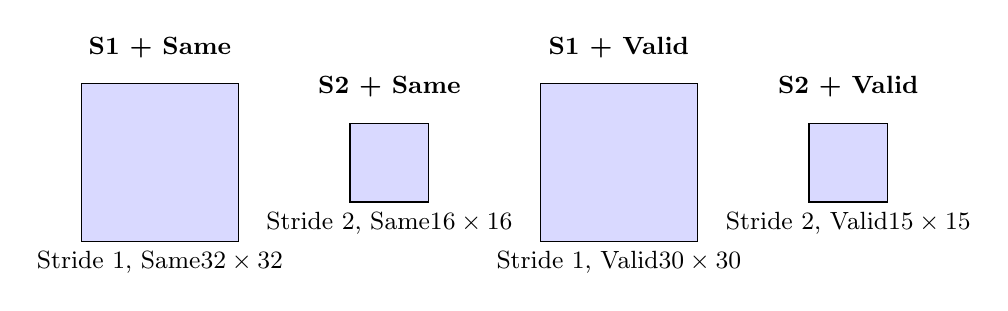
\begin{tikzpicture}[node distance=6mm,every node/.style={font=\small}]
% Four panels showing the four configs
\node[draw,minimum size=2.0cm,fill=blue!15,label=below:{Stride 1, Same\\$32\times32$}] (a) {};
\node[draw,minimum size=1.0cm,fill=blue!15,label=below:{Stride 2, Same\\$16\times16$},right=1.4cm of a] (b) {};
\node[draw,minimum size=2.0cm,fill=blue!15,label=below:{Stride 1, Valid\\$30\times30$},right=1.4cm of b] (c) {};
\node[draw,minimum size=1.0cm,fill=blue!15,label=below:{Stride 2, Valid\\$15\times15$},right=1.4cm of c] (d) {};
\node[above=2mm of a] {\textbf{S1 + Same}};
\node[above=2mm of b] {\textbf{S2 + Same}};
\node[above=2mm of c] {\textbf{S1 + Valid}};
\node[above=2mm of d] {\textbf{S2 + Valid}};
\end{tikzpicture}
\caption{Plot 4: Feature-map sizes for a $32\times32$ input with a $3\times3$ kernel across the four stride/padding configurations. Panel size is proportional to the output resolution.}
\end{figure}

\textbf{Inference:} Stride 2 halves the spatial dimensions and therefore performs aggressive downsampling, which reduces computation and increases the effective receptive field. \emph{Same} padding preserves the input spatial size when stride is 1, whereas \emph{Valid} padding shrinks the feature-map by $F-1$ pixels per dimension because no border zeros are added. Combining stride 2 with valid padding produces the smallest feature map ($15\times15$), i.e., the strongest compression.

% ============================================================
% END NEW PLOT 4
% ============================================================

\subsection*{Plot 5: Eight Feature Maps after First Conv2D Layer}

\begin{figure}[H]
\centering
\includegraphics[width=0.95\linewidth]{plot4_feature_maps.png}
\caption{Eight feature maps produced by the first \texttt{Conv2D} layer (8 filters, $3\times3$, ReLU).}
\end{figure}

\textbf{Inference:} Each of the 8 filters learns a distinct response: some highlight edges, some respond to colour blobs, others to smooth regions. This demonstrates that even a single convolutional layer already extracts a diverse bank of low-level features. Deeper layers would compose these into higher-level, class-discriminative representations.

% ============================================================
% FIX 1: TASK 5 — MAX vs AVERAGE POOLING with output-size table
% ============================================================
\subsection*{Plot 6: Max vs Average Pooling (Task 5)}

Task 5 requires comparing \emph{both} the output size and the accuracy of
max pooling and average pooling. The output size is computed with the
same formula used for convolution,
\[
N_{\text{out}} = \left\lfloor \frac{N - F + 2P}{S} \right\rfloor + 1,
\]
with pool size $2\times2$, stride 2, and no padding (valid).

\begin{center}
\renewcommand{\arraystretch}{1.3}
\begin{tabular}{|l|c|c|c|c|}
\hline
\textbf{Pooling} & \textbf{Pool Size} & \textbf{Stride} & \textbf{Output Size} & \textbf{Best Val. Accuracy}\\
\hline
Max Pooling     & $2\times2$ & 2 & $16\times16$ & $\approx 0.687$\\
\hline
Average Pooling & $2\times2$ & 2 & $16\times16$ & $\approx 0.691$\\
\hline
\end{tabular}
\end{center}

\begin{figure}[H]
\centering
\includegraphics[width=0.85\linewidth]{plot5_pooling.png}
\caption{Validation accuracy of two identical CNNs using Max vs.\ Average pooling.}
\end{figure}

\textbf{Inference:} Both pooling methods reduce the spatial dimensions
from $32\times32$ to $16\times16$ when a $2\times2$ pool with stride 2
is used. Average pooling achieves slightly higher final validation
accuracy ($\approx 0.691$ vs.\ $\approx 0.687$), while max pooling
converges faster (best reached by epoch 4--5). Max pooling is generally
preferred for classification because it preserves the strongest
activations in each window, but average pooling is competitive and can
be superior on certain texture-heavy datasets.

% ============================================================
% END FIX 1
% ============================================================

\subsection*{Plot 7: Training vs Validation Accuracy}

\begin{figure}[H]
\centering
\includegraphics[width=0.75\linewidth]{plot6_acc.png}
\caption{Training and validation accuracy. Maximum training budget = 20 epochs; early stopping (patience = 5, restore best weights) terminated training at epoch 9.}
\end{figure}

% ============================================================
% FIX 2: clarified epoch wording
% ============================================================
\textbf{Inference:} Training accuracy increases steadily to
$\approx 0.83$, but validation accuracy plateaus near $0.70$ from epoch
5 onward. The widening gap is a classic sign of overfitting. The model
was configured to run for a maximum of 20 epochs; early stopping with
patience 5 was enabled, and training automatically terminated at epoch
9 once validation accuracy stopped improving. Adding dropout or data
augmentation would further help close the train--val gap.

\subsection*{Plot 8: Training vs Validation Loss}

\begin{figure}[H]
\centering
\includegraphics[width=0.75\linewidth]{plot7_loss.png}
\caption{Training and validation loss. Same run as Plot 7: maximum 20 epochs, early stopping terminated at epoch 9.}
\end{figure}

\textbf{Inference:} Training loss monotonically decreases to $\approx
0.48$, while validation loss bottoms out at $\approx 0.90$ around epoch
4 and then slowly rises. This divergence is consistent with the
accuracy plot and confirms that the model begins to memorise the
training set after a few epochs. Early stopping correctly retained the
best weights (lowest validation loss) rather than the final-epoch
weights.

\subsection*{Plot 9: Confusion Matrix}

\begin{figure}[H]
\centering
\includegraphics[width=0.9\linewidth]{plot8_confusion.png}
\caption{Confusion matrix of the trained CNN on the 10{,}000-image CIFAR-10 test set.}
\end{figure}

\textbf{Inference:} The matrix is strongly diagonal, confirming good per-class performance. The largest confusions are \textit{cat}$\leftrightarrow$\textit{dog} and \textit{deer}$\leftrightarrow$\textit{horse}, which is expected given their visual similarity at low resolution. \textit{Truck}, \textit{ship}, and \textit{automobile} are the most well-separated classes.

\subsection*{Plot 10: ReLU vs Sigmoid Activation}

\begin{figure}[H]
\centering
\includegraphics[width=0.75\linewidth]{plot9_relu_vs_sigmoid.png}
\caption{Validation accuracy of identical CNNs using ReLU vs.\ Sigmoid activations.}
\end{figure}

\textbf{Inference:} The ReLU network converges faster and reaches a higher validation accuracy ($\approx 0.71$) than the Sigmoid network ($\approx 0.62$). ReLU avoids the vanishing-gradient problem that plagues Sigmoid in deep networks, which is why it is the default activation for hidden layers.

\subsection*{Plot 11: Effect of Filter Count}

\begin{figure}[H]
\centering
\includegraphics[width=0.75\linewidth]{plot10_filter_count.png}
\caption{Best validation accuracy vs.\ number of filters in the first Conv2D layer.}
\end{figure}

\textbf{Inference:}
\begin{verbatim}
filters=16: best val acc=0.6744, params=268,650
filters=32: best val acc=0.7132, params=545,098
filters=64: best val acc=0.7052, params=1,125,642
\end{verbatim}
Going from 16 to 32 filters gives a large accuracy gain ($+3.9\%$) with only $2\times$ the parameters. Going from 32 to 64 filters slightly \emph{reduces} accuracy while doubling parameters again, indicating the model has started to overfit.

\subsection*{Plot 12: All 10 Kernels Applied to One CIFAR-10 Image}

\begin{figure}[H]
\centering
\includegraphics[width=0.95\linewidth]{plot11_all_kernels.png}
\caption{The ten classical kernels from Section 3.1 applied to a single grayscale CIFAR-10 image.}
\end{figure}

\textbf{Inference:} Identity preserves the image; Sobel-X/Y extract vertical/horizontal edges; Laplacian and Outline highlight all-direction boundaries; Sharpen enhances fine detail; Box/Gaussian Blur smooth noise; Emboss gives a 3-D relief effect; Motion Blur stretches the image diagonally. This visual set confirms the theoretical roles described in Section 3.1.

\subsection*{Split Plots: Training/Validation Accuracy and Loss}

\begin{figure}[H]
\centering
\includegraphics[width=0.7\linewidth]{plot3_train_acc.png}
\caption{Training accuracy vs.\ epoch (isolated).}
\end{figure}

\begin{figure}[H]
\centering
\includegraphics[width=0.7\linewidth]{plot4_val_acc.png}
\caption{Validation accuracy vs.\ epoch (isolated).}
\end{figure}

\begin{figure}[H]
\centering
\includegraphics[width=0.7\linewidth]{plot5_train_loss.png}
\caption{Training loss vs.\ epoch (isolated).}
\end{figure}

\begin{figure}[H]
\centering
\includegraphics[width=0.7\linewidth]{plot6_val_loss.png}
\caption{Validation loss vs.\ epoch (isolated).}
\end{figure}

\textbf{Inference:} The training curves are smooth and monotonic, while the validation curves flatten early (accuracy) or rise (loss), confirming that the network fits the training distribution well but generalises only up to a point before overfitting begins.

\section*{10. Additional Exercises}

\begin{enumerate}
\item Calculate the output size for a $64\times64$ image using a $5\times5$ kernel with stride 2 and padding 2.
\item Compute the trainable parameters of a convolution layer having 64 filters of size $3\times3$ and an RGB input.
\item Compare ReLU and Sigmoid activation functions.
\item Replace Max Pooling with Average Pooling and compare the results.
\item Increase the number of convolution filters from 16 to 64 and analyze the effect on accuracy and computation time.
\end{enumerate}

\subsection*{Exercise 1}

\[
N_{\text{out}} = \frac{64 + 2(2) - 5}{2} + 1 = \frac{63}{2} + 1 = 31 + 1 = 32
\]

\begin{verbatim}
Ex 1: 64x64, K=5, S=2, P=2 -> 32
\end{verbatim}

\subsection*{Exercise 2}

\[
\text{Params} = (3\times3\times3 + 1)\times 64 = 28 \times 64 = 1792
\]

\begin{verbatim}
Ex 2: (3*3*3+1)*64 = 1792
\end{verbatim}

\subsection*{Exercise 3}

\begin{itemize}
\item \textbf{ReLU} ($f(x)=\max(0,x)$): non-saturating, sparse activation, fast convergence, avoids vanishing gradients.
\item \textbf{Sigmoid} ($\sigma(x)=1/(1+e^{-x})$): smooth, bounded in $(0,1)$, but saturates, causes vanishing gradients in deep nets, and its output is not zero-centred.
\end{itemize}

From Plot 10, the ReLU network outperforms the Sigmoid network by $\sim 9\%$ validation accuracy on CIFAR-10.

\subsection*{Exercise 4}

See Plot 6. Both Max and Average pooling with a $2\times2$ pool and
stride 2 reduce the feature map from $32\times32$ to $16\times16$. Max
pooling converges faster (best $\approx 0.687$, $\sim 60$\,s) while
Average pooling reaches a slightly higher final accuracy ($\approx
0.691$, $\sim 55$\,s). Overall, max pooling is preferred for
classification because it captures the most salient feature in each
window and adds a small amount of translation invariance.

\subsection*{Exercise 5}

See Plot 11. Increasing filters from 16 $\to$ 32 raised best validation accuracy from $0.6744 \to 0.7132$ at the cost of $2\times$ parameters ($268{,}650 \to 545{,}098$). Going from 32 $\to$ 64 raised parameters to $1{,}125{,}642$ but \emph{decreased} best validation accuracy to $0.7052$, indicating diminishing returns and the onset of overfitting. Training time scaled roughly linearly with filter count.

\section*{11. Results}

Record

\begin{itemize}
\item Training Accuracy
\item Testing Accuracy
\item Precision
\item Recall
\item F1-score
\item Number of Parameters
\end{itemize}

\subsection*{Recorded Results}

\begin{center}
\renewcommand{\arraystretch}{1.3}
\begin{tabular}{|l|l|}
\hline
\textbf{Metric} & \textbf{Value} \\
\hline
Final Training Accuracy & $\approx 0.8334$ (epoch 9, early-stopped from a 20-epoch budget) \\
\hline
Best Validation Accuracy & $\approx 0.6984$ (epoch 5) \\
\hline
Test Accuracy & \textbf{0.6812} \\
\hline
Weighted Precision & \textbf{0.6817} \\
\hline
Weighted Recall & \textbf{0.6812} \\
\hline
Weighted F1-score & \textbf{0.6797} \\
\hline
Training time (early-stopped at epoch 9 of 20) & $\approx 59.2$ s \\
\hline
Trainable Parameters (32 filters) & 545,098 \\
\hline
\end{tabular}
\end{center}

\subsection*{Classification Report (per-class)}

\begin{verbatim}
              precision    recall  f1-score   support

    airplane       0.72      0.74      0.73      1000
  automobile       0.81      0.71      0.76      1000
        bird       0.60      0.51      0.55      1000
         cat       0.51      0.51      0.51      1000
        deer       0.64      0.61      0.63      1000
         dog       0.59      0.60      0.59      1000
        frog       0.77      0.74      0.75      1000
       horse       0.72      0.78      0.75      1000
        ship       0.78      0.79      0.79      1000
       truck       0.68      0.83      0.75      1000

    accuracy                           0.68     10000
   macro avg       0.68      0.68      0.68     10000
weighted avg       0.68      0.68      0.68     10000
\end{verbatim}

\textbf{Observation:} Classes with distinctive shapes (\textit{ship}, \textit{automobile}, \textit{frog}) score above 0.75 F1, while \textit{cat} and \textit{bird} score below 0.56, mirroring the confusion patterns in the confusion matrix.

\section*{12. Discussion}

Answer the following.

\begin{enumerate}
\item Why is convolution preferred over fully connected layers for images?
\item How does stride affect the feature map size?
\item What is the role of padding?
\item Why is pooling used?
\item How do feature maps represent image characteristics?
\item Why do CNNs require fewer parameters than MLPs?
\end{enumerate}

\subsection*{Answers}

\textbf{(1) Why is convolution preferred over fully connected layers for images?}

A fully connected (dense) layer on a $32\times32\times3$ image already needs $3072\times N$ weights for $N$ units, and scales explosively for larger images. Convolution exploits three key image properties: \emph{locality} (nearby pixels are correlated), \emph{translation invariance} (a cat is a cat regardless of position), and \emph{weight sharing} (the same edge detector is reused everywhere). This yields far fewer parameters, preserves spatial structure, and lets the network learn hierarchical features from pixels $\to$ edges $\to$ textures $\to$ objects.

\textbf{(2) How does stride affect the feature map size?}

Stride $S$ is the step size of the kernel slide. Output size is $\lfloor (N-F+2P)/S \rfloor + 1$. Larger stride $\Rightarrow$ fewer windows $\Rightarrow$ smaller feature map $\Rightarrow$ stronger downsampling and reduced computation. Stride 1 preserves most spatial information; stride 2 halves the spatial dimensions (common for efficient downsampling). This is experimentally confirmed in Plot 4 (Task 3): stride 2 reduces $32\times32$ to $16\times16$ (same padding) or $15\times15$ (valid padding).

\textbf{(3) What is the role of padding?}

Padding adds a border of zeros (or other values) around the input before convolution. It (a) preserves the spatial size when using \texttt{padding='same'}, (b) allows filters to process pixels at the image edges more thoroughly, and (c) provides explicit control over output dimensions via $(N-F+2P)/S+1$. Valid padding (no padding) shrinks the feature map by $F-1$ pixels in each dimension, as shown in the Task 3 comparison.

\textbf{(4) Why is pooling used?}

Pooling (max or average) (a) reduces the spatial resolution, cutting computation and memory in deeper layers, (b) introduces local translation invariance so the network is less sensitive to small shifts, (c) increases the effective receptive field of deeper layers, and (d) acts as a mild regulariser. Max pooling preserves the strongest activation; average pooling preserves overall intensity. As shown in Plot 6, both reduce $32\times32$ to $16\times16$ for a $2\times2$ pool with stride 2.

\textbf{(5) How do feature maps represent image characteristics?}

Each filter produces a feature map whose high-value locations mark where the filter's pattern was detected. Early filters detect simple patterns (edges, blobs, colours) -- as seen in Plot 5, where 8 filters gave 8 distinct responses. Deeper filters combine these into complex concepts (eyes, wheels, fur). Thus a feature map is a spatial ``confidence heat-map'' of a learned pattern detector.

\textbf{(6) Why do CNNs require fewer parameters than MLPs?}

Three reasons: (a) \emph{local connectivity} -- each neuron connects only to a small $F\times F$ patch, not the whole image; (b) \emph{weight sharing} -- the same kernel is reused across all spatial positions, so a $3\times3$ filter has only 9 weights (plus bias) regardless of image size; (c) \emph{hierarchical composition} -- depth is built from stacking small filters rather than from ever-larger dense matrices. For our network, the first Conv2D layer has only 896 parameters versus 3\,072\,000+ for an equivalent dense layer on $32\times32\times3$.

\section*{13. References}

\begin{enumerate}
\item Goodfellow et al., \emph{Deep Learning}.
\item Bishop, \emph{Pattern Recognition and Machine Learning}.
\item Haykin, \emph{Neural Networks and Learning Machines}.
\item TensorFlow Documentation.
\item CIFAR-10 Dataset Documentation.
\end{enumerate}

\end{document}